\documentclass[a4paper, 11pt]{article}

\usepackage{graphicx}
\usepackage{tocloft}
\usepackage{xcolor}
\usepackage{hyperref}
\usepackage{amsmath} % for math notation
\usepackage{listings} % for code blocks
\usepackage{graphicx} % for images
\usepackage[T1]{fontenc}
\usepackage[utf8]{inputenc}
\usepackage[german]{babel}
\usepackage{datetime2}
\DTMsetdatestyle{german}

\lstdefinestyle{code}{
  basicstyle=\fontsize{10pt}{10pt}\selectfont\ttfamily, % set the font
  breaklines=true,      % Automatically break lines
  language=Python,
}

\begin{document}
\pagenumbering{roman}

\selectlanguage{ngerman}
\begin{titlepage}
    \begin{flushleft}
        Software Engineering -- ERP-Systeme (Frank Mysliwitz)\\

        \huge
        \textbf{KI gestützte Stammdatenprüfung: Gefahrengut}\\
        \vspace{1,5cm}

        \Large
        \textbf{Dominik Agreš} {\small (?)}\\
        \textbf{Chris Kiriakou} {\small (209385)}\\
        \textbf{David Koch} {\small (212824)}\\
        \textbf{Berkan Nur} {\small (?)}\\
        \vspace{1,5cm}
        
        \large
        \section*{Vorwort}
        In diesem Bericht wird die Vorgehensweise zur Semesteraufgabe beschrieben.
        Das Ziel war es, mithilfe von künstlicher Intelligenz, Fehler in den Stammdaten zu
        finden. Hierfür wird eine Einführung in das Gefahrengut geben. Anschließend werden
        drei Ansätze zur Püfung des Gefahrenguts aufgezeigt. 
        Die zum Projekt geschriebene Software befindet sich in einem öffentlich 
        zugänglichen \href{https://github.com/ckiri/wetterstation}{\textcolor{blue}{Repository}}.\\

        \vspace{2,5cm}

        \today \\

        \vspace{3,5cm}
    \end{flushleft}
\end{titlepage}


\newpage

\setcounter{tocdepth}{2}
\addcontentsline{toc}{section}{Inhaltsverzeichnis}
\tableofcontents

\newpage

% % David
\section{Gefahrengüter}


\newpage

% % Chris
\section{Automatische Stammdatenprüfung}

Im ersten Ansatz werden die Daten des Gefahrenguts analysiert und versucht ohne
Einsatz von künstlicher Intelligenz Fehler zu erkennen. Hierfür wird zuerst
eine Bezeichnungsanalyse durchgeführt. Dabei wird die Spalte
\textbf{Material-Bezeichnung} der Stammdaten betrachtet und mit der Spalte
\textbf{Bezeichnung} der UN-Nummern Liste verglichen.\\

Für die Datenanalyse bietet sich Python dank seines umfangreichen Ökosystems 
gut an. Um die Datenanalyse interaktiv zu gestalten wird ein Jupyter Notebook
verwendet.\\

In diesem Kapitel werden folgende Python Bibliotheken verwendet:
\begin{itemize}
    \item Pandas
    \item Matplotlib
    \item Openpyxl
\end{itemize}

\textbf{Pandas} ist eine Open-Source-Bibliothek für Python, die speziell für die
Datenanalyse und -manipulation entwickelt wurde. Hier ist besonders die 
Datenstruktur \textbf{DataFrame} von großer Bedeutung. Diese ist eine
zweidimensionale Tabelle mit Zeilen- und Spaltenbeschriftungen, ähnlich wie bei
einer Excel-Tabelle. Mit Pandas lassen sich Daten aus verschiedenen Quellen wie
CSV-, Excel- oder JSON-Dateien bequem einlesen und weiterverarbeiten.
Außerdem kann Pandas auch HTML-Dateien mithilfe von \textbf{lxml} einlesen und
in einen Dataframe konvertieren. Dabei parst lxml Tabellen, also den
HTML-Tabellentag \texttt{<table>...</table>}, innherhalb eines HTML-Dokuments.
\textbf{Matplotlib} erlaubt es uns die vorhandenen und extrahierten Daten
visuell darzustellen. Dies kann das Verständnis komplexer Zusammenhänge 
vereinfachen.
Pandas ist durchaus fähig Excel-Dateien zu verarbeiten. Formatierungen und 
Formeln in den Zellen werden aber nicht übernommen. Hier kommt \textbf{Openpyxl}
zum Einsatz. Diese Bibliothek erlaubt es uns die Daten im in einer neuen Tabelle
mit der identischen Formatierung wieder abzuspeichern.\\

In diesem Kapitel wird dieses 
\href{https://github.com/ckiri/gg/tree/master/notebooks/automatic_error_detection.ipynb}
{\textcolor{blue}{Jupyter Notebook}} verwendet und beschrieben.

\newpage

\subsection{Bezeichnungsanalyse}

Als Datenbasis wird die UN-Nummer-Liste von Wikipedia verwendet. Es sei hierbei
noch zu erwähnen, dass es hierfür auch Datenbanken und Tabellen gibt
(teilweise Gebührenpflichtig). Die Liste auf Wikipedia kann aber, wie bereits 
erwähnt, mit wenig aufwand in Pandas verwendet werden. Für die
Bezeichnungsanalyse wird vorerst aber nur die Bezeichner-Spalte relevant sein,
da hier semantische Beziehungen zur \textbf{Material-Bezeichnung} hergestellt
werden.\\

\subsubsection{Laden UN-Nummer-Liste}

Folgender Code lädt und speichert die UN-Nummer-Liste in einen Pandas Dataframe.
Nach erfolgreichem Laden der Tabelle wird die Spalte \textbf{'Bezeichnung'} in
die Variable \texttt{un\_numbers\_designation\_col} geladen. Da die 
UN-Nummer-Liste in mehrere Tabellen unterteilt ist werden diese mit
\texttt{.concat()} zuvor noch konkatiert:\\

\begin{lstlisting}
un_numbers_filename = "un_numbers_wikipedia.html"
un_numbers_html_path = os.path.join(data_path, un_numbers_filename)
un_numbers_url = "https://de.wikipedia.org/wiki/Liste_der_UN-Nummern"

if not os.path.exists(un_numbers_html_path):
    try:
        print("Downloading UN number table ...")

        response = requests.get(un_numbers_url)
        response.raise_for_status()

        with open(
            un_numbers_html_path,
            "w",
            encoding="utf-8"
        ) as f:
            f.write(response.text)

        print(f"Saved HTML to {un_numbers_html_path}")

    except Exception as e:
        print(f"Failed to fetch HTML page: {e}")

un_numbers_tables = pd.read_html(un_numbers_html_path)
un_numbers_df = pd.concat(un_numbers_tables).reset_index(drop=True)
un_numbers_designation_col = un_numbers_df['Bezeichnung']
\end{lstlisting}

\newpage

\subsubsection{Laden Stammdaten}

Im nächsten Schritt werden die Stammdaten, ähnlich wie die UN-Nummer-Liste
in einen Dataframe geladen. Erwähnenswert hierbei ist noch, dass die geladene
Excel-Datei eine nicht zu vernachlässigende Größe von $12715 \times 111$ Zellen
hat. Daher kann der Ladevorgang je nach Hardware einen kurzen Augenblick dauern.
Die ersten drei Spalten der Stammdaten beinhalten keine relevanten
Informationen, daher müssen diese also nicht geladen werden.\\

Mit Openpyxl wird nun \textbf{Tabelle1} in den Stammdaten in die
Variable \texttt{ws} \textit{(Worksheet)} geladen. Dies wird für den Schluss
relevant werden, da hier die korrigierten Daten wieder eingefügt werden. Mit
Pandas werden die Stammdaten in den \texttt{full\_df}-Dataframe geladen. Wie bei
Openpyxl werden die ersten drei Zeilen nicht benötigt. Die vierte hingegen
wird als Header verwendet. Danach wird die Spalte
\textbf{Material-Bezeichnung} der Variable \texttt{masterdata\_designation\_col}
zugewiesen:\\

\begin{lstlisting}
md_filename = "stammdaten.xlsx"
masterdata_path = os.path.join(data_path, md_filename)

wb = openpyxl.load_workbook(masterdata_path)
ws = wb['Tabelle1']

for row in ws.iter_rows(min_row=4, max_row=ws.max_row):
    for cell in row:
        cell.value = None

full_df = pd.read_excel(masterdata_path, header=None)
skipped_info = full_df.iloc[:2]
md_df = full_df.iloc[2:]
md_df.columns = md_df.iloc[0] 
md_df = md_df[1:].reset_index(drop=True)
md_designation_col = md_df['Material-Bezeichnung']
\end{lstlisting}

\subsubsection{Analyse Bezeichnungsfelder}

In diesem Teil findet die eigentliche Analyse zur semantische Beziehung der
Feldern der \textbf{Material-Bezeichnung} in den Stammdaten mit den Bezeichnern
der UN-Nummern statt. Durch das Erstellen der Beziehungen können dann
Materialien der Modulgruppen den UN-Nummern zugeordnet werden. 
\newpage

Zuerst ist es aber notwendig die Bezeichnungsfelder zu bereiningen. In den
Stammdaten kommen keien Umlaute (ä, ö, ü) vor. Ebenfalls sollen unnötige 
Satzzeichen entfernt werden. Nach der Normalisierung wird die Häufigkeit der
verwendeter Wörter ermittelt:\\

\begin{lstlisting}
masterdata_designation_words = []
un_numbers_designation_words = []

def normalize_text(text):
    if pd.isna(text):
        return []
    cleaned = (
        text.lower()
        .replace('ae', 'ä')
        .replace('oe', 'ö')
        .replace('ue', 'ü')
        .replace('.', '')
        .replace(',', '')
    )
    return cleaned.split()

masterdata_designation_words.extend(
    md_designation_col
        .dropna()
        .apply(normalize_text)
        .explode()
)

un_numbers_designation_words.extend(
    un_numbers_designation_col
        .dropna()
        .apply(normalize_text)
        .explode()
)
\end{lstlisting}

\newpage

Mithilfe von Matplotlib lassen sich die 50 häufigsten Wörter, wie in
Abb.~\ref{fig:top-50-unfiltered} visuell darstellen. Dabei wird sichtbar warum
ein anschließendes Bereinigen der Bezeichnungsfelder notwendig ist:\\

\begin{lstlisting}
def plot_wc(title, all_words):

    word_counts = Counter(all_words)
    top_n = 50
    top_words = word_counts.most_common(top_n)
    words, counts = zip(*top_words)

    plt.figure(figsize=(12, 6))
    plt.bar(words, counts, color='steelblue')
    plt.xticks(rotation=45, ha='right')
    plt.ylabel("Häufigkeit")
    plt.title(f"Die {top_n} häufigsten Wörter in {title}")
    plt.tight_layout()
    plt.show()

plot_wc("Stammdaten", masterdata_designation_words)
plot_wc("UN-Nummern", un_numbers_designation_words)
\end{lstlisting}

\begin{figure}[htbp]
  \centering
  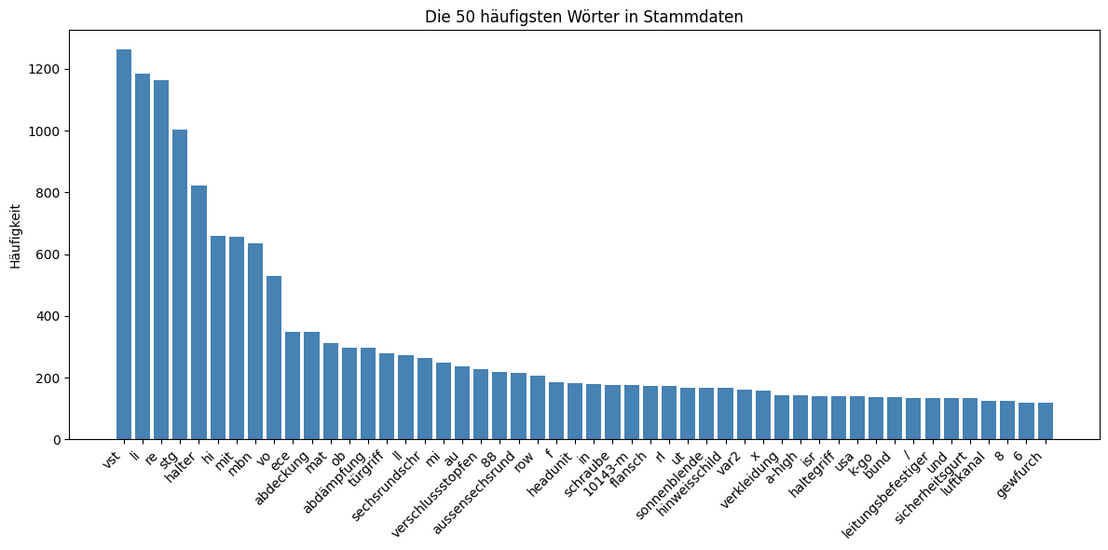
\includegraphics[width=0.8\textwidth]{gg-top-50-words-masterdata.png}
  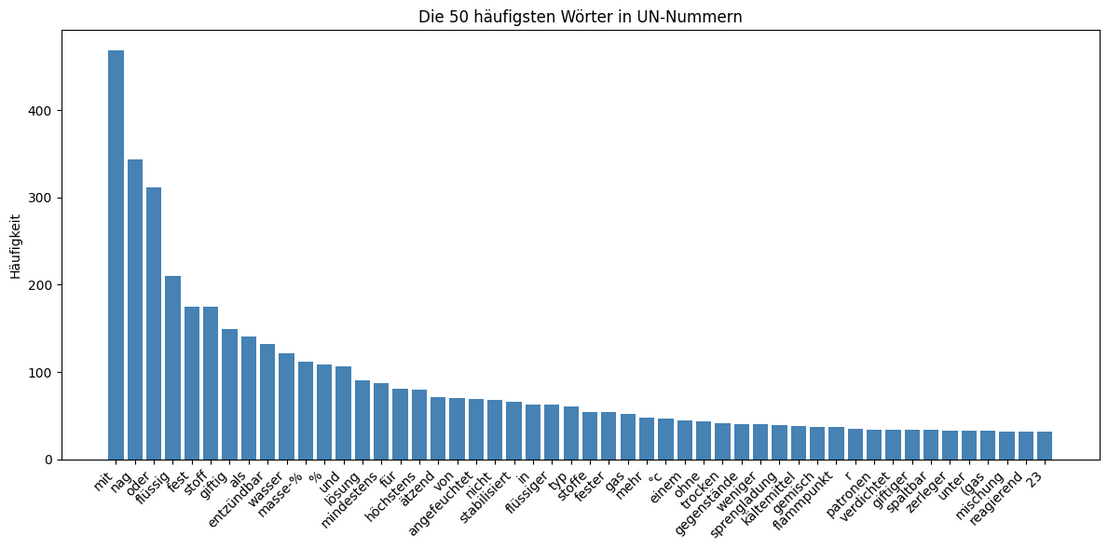
\includegraphics[width=0.8\textwidth]{gg-top-50-words-un-numbers.png}
  \caption{Top 50 Wörter beider Bezeichnungsspalten \textit{(ungbereinigt)}}
  \label{fig:top-50-unfiltered}
\end{figure}

\newpage

Für ein effizienteres Verarbeiten der Daten ist es notwendig das Grundrauschen
zu entfernen. Mit Grundrauschen sind vorallem Wörter gemeint, die keine
semantische Relevanz haben. Hierzu wurde manuell eine Liste an sogenannten
\texttt{stop\_words} definiert. Ist die Filterung abgeschlossen, erhält man,
wie in Abb.~\ref{fig:top-50-filtered}, Listen von Schlüsselwörtern
jeder Spalte:\\

\begin{lstlisting}
def sanitize_text(text):
    if not isinstance(text, str):
        return set()
    text = (
        text.lower()
        .replace('li-ion', 'lithium-ionen')
        .replace('bat.', 'batterie')
    )
    words = set(text.split())
    cleaned_words = {
        word for word in words
        if word not in stop_words
        and not re.search(r'\d', word)
        and len(word) >= 3
    }

    return cleaned_words
\end{lstlisting}

\begin{figure}[htbp]
  \centering
  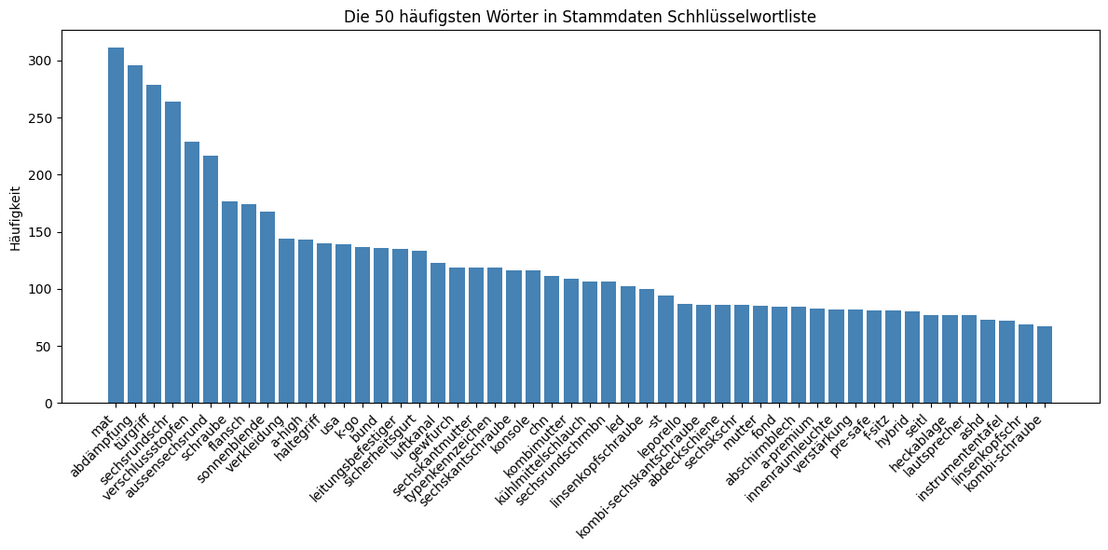
\includegraphics[width=0.8\textwidth]{gg-top-50-words-masterdata-keywords.png}
  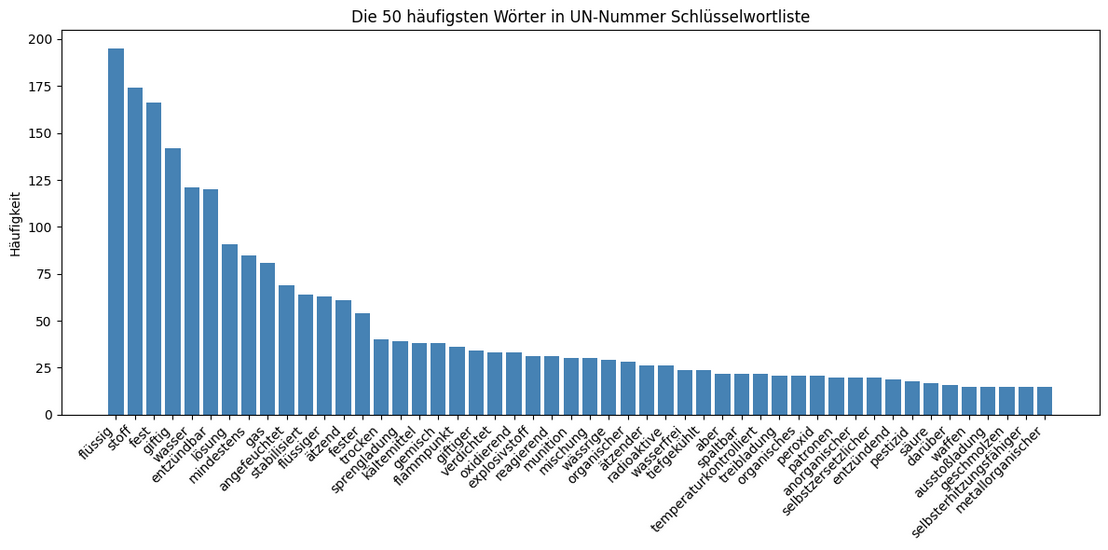
\includegraphics[width=0.8\textwidth]{gg-top-50-words-un-numbers-keywords.png}
  \caption{Top 50 Wörter beider Bezeichnungsspalten \textit{(bereinigit)}}
  \label{fig:top-50-filtered}
\end{figure}

\newpage

\subsubsection{Beziehung der Bezeichner} 

Durch das Vergleichen jedes einzelnen Schlüsselworts aus der Spalte
\textbf{Material-Bezeichnung} mit allen Schlüsselwörtern der UN-Nummern
Bezeichnungen kann festgestellt werden welche Zeilen welchen der UN-Nummer-Liste
ähneln. Dieses Verfahren hat eine Laufzeitkomplexität von $m \times n$ und 
ist daher nicht optimal obwohl bereits eine Filterung angewendet wurde.
Was zusätzlich die Effizienz beinträchtigt ist der verwendete Fuzzy-Algorithmus
der gleiche Substrings der Schlüsselwörter ermittelt:\\

\begin{lstlisting}
for un_idx, un_words in un_keywords_col.items():
    local_match = set()

    for mw in master_words:
        for uw in un_words:
            if len(mw) >= 4
                    and len(uw) >= 4
                    and (mw in uw or uw in mw):
                local_match.add(f"{mw} <-> {uw}")
            elif partial_ratio(mw, uw) > 85:
                local_match.add(f"{mw} <~> {uw}")

\end{lstlisting}

\begin{figure}[htbp]
  \centering
  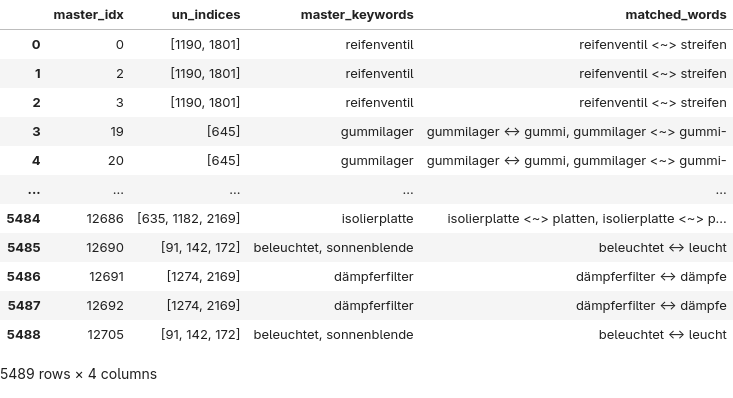
\includegraphics[width=0.8\textwidth]{gg-designation-analysis.png}
  \caption{Beziehung der Schlüsselwörter in Bezeichnerspalten}
  \label{fig:designation}
\end{figure}

In Abb.~\ref{fig:designation} fällt auf, das Materialbezeichner nicht
100\%-tig auf die Bezeichnungen der UN-Nummern zugeordnet werden können.
Außerdem kann durch diese Methode auch nicht der Kontext betrachtet werden.
Die Bezeichungsanalyse ist somit nicht der richtige Ansatz.

\newpage

\subsection{Erkennenung von Unregelmäßigkeiten}

Es sollen nun Unregelmäßigkeiten beim Gefahrengut erkannt werden. Dabei werden
nur die für das Gefahrengut relevanten Spalten betrachtet. Hierfür schauen wir
uns zuerst an, ob in der Spalte \texttt{Art\_IdentNr} der Wert \texttt{UN}
gesetzt ist. Ist dies der Fall, nehmen wir aus der Spalte
\textbf{Material-Bezeichnung} der gleichen Zeile das erste Wort. Mit diesem Wort
werden alle nachträglichen Reihen der \textbf{Material-Bezeichnung} die jeweils
mit dem gleichen Wort beginnen, durchsucht. Ist hierbei die Spalte
\texttt{Art\_IdentNr} nicht mit dem Wert \texttt{UN} gesetzt so haben wir eine
Unregelmäßigkeit festgestellt. Dieses Verfahren wird mithilfe von Masken
umgesetzt bei denen gesetzte und ungesetzte Zeilen der Spalte
\texttt{Art\_IdentNr} verundet werden:\\

\begin{lstlisting}
for first_word, group in grouped:
    un_mask = group['Art_IdentNr'] == 'UN'
    non_un_mask = group['Art_IdentNr'] != 'UN'

    has_un = un_mask.any()
    has_non_un = non_un_mask.any()

    if has_un and has_non_un:
        inconsistent_first_words.append(first_word)
        for idx, row in group.iterrows():
            is_correct = row['Art_IdentNr'] == 'UN'
            row_dict = row.to_dict()
            row_dict['Korrektheit'] = is_correct
            row_dict['Ursprungsindex'] = idx  
            rows.append(row_dict)
\end{lstlisting}

In Abb.~\ref{fig:automatic-error-detection} ist zu sehen, dass Gruppen bei denen
Unregelmäßigkeiten vorkommen, dargestellt werden. Bei Korrektheit sind die
Zeilen grün gefärbt. Zeilen in denen eine Diskrepanz vorliegt sind rot gefärbt.
Hierbei wurde die Annahme getroffen, dass die Daten mit ausgefüllter
\texttt{Art\_IdentNr} korrekt ausgefüllt wurden.

\begin{figure}[htbp]
  \centering
  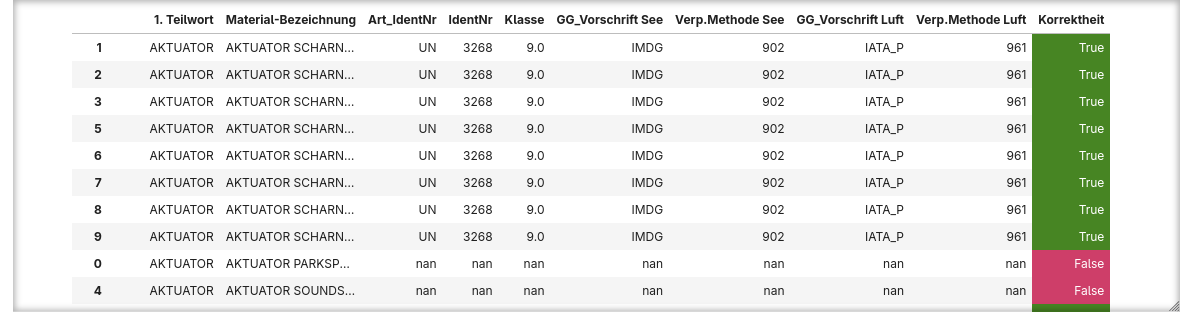
\includegraphics[width=0.8\textwidth]{gg-inconsistency-detection.png}
  \caption{Erkannte Unregelmäßigkeiten}
  \label{fig:automatic-error-detection}
\end{figure}

\newpage

\subsection{Fazit automatische Stammdatenprüfung}

Leider hatten beide Ansätze nicht die gewünschte Aussagekraft. Selbst bei der
Bildung von Wortgruppen kommt es zu Fehlern. Als Beispiel kann hier die
Gruppe \textbf{AKTUATOR} aufgeführt werden. Es wurde, wie in
Abb.~\ref{fig:automatic-error-detetction} zu sehen, auch ein
\textbf{AKTUATOR SOUNDSYSTEM} fälschlicherweise als Gefahrengut angesehen.
Ein Lautsprecher ist aber auf keinen Fall ein Gefahrengut. Wie man hieraus
erkennen kann ist es unabdingbar den Kontext der einzelnen Objekte zu
betrachten. In den nächsten Abschnitten wird mithilfe eines KI basierten
Ansatz eben genau dieses Problem geprüft.




\newpage

% % Berkan
\section{KI basierter Ansatz}


\newpage

% % Dominik
\section{Fehlererkennung mit ML}


\newpage

\addcontentsline{toc}{section}{Abbildungsverzeichnis}
\listoffigures

\newpage

\addcontentsline{toc}{section}{Literature}
%\printbibliography

\end{document}
